\documentclass{beamer}

\usepackage{siunitx}
\usepackage{subcaption}
\usepackage[american]{circuitikz}
\usepackage{threeparttable}
\usepackage{tikz}
\usepackage{pgfplots}
\usepackage{multirow}

\usetheme{Boadilla}

\setbeamertemplate{bibliography item}{[\arabic{enumiv}]}
\usepackage{caption}
\captionsetup[figure]{labelformat=empty}
\captionsetup[subfigure]{labelformat=empty}
\captionsetup[table]{labelformat=empty}

\beamertemplatenavigationsymbolsempty

\author{Miguel Perez Andrade}
\title{Tesis de grado}
\subtitle{Diseño de un generador de pulsos ultracortos}
\date{12 de diciembre de 2023}
\institute{Facultad de Ingeniería de la Universidad de Buenos Aires}

\makeatletter
\setbeamertemplate{footline}
{
  \leavevmode%
  \hbox{%
  \begin{beamercolorbox}[wd=.333333\paperwidth,ht=2.25ex,dp=1ex,center]{author in head/foot}%
    \usebeamerfont{author in head/foot}\insertshortauthor
  \end{beamercolorbox}%
  \begin{beamercolorbox}[wd=.333333\paperwidth,ht=2.25ex,dp=1ex,center]{title in head/foot}%
    \usebeamerfont{title in head/foot}\insertshorttitle
  \end{beamercolorbox}%
  \begin{beamercolorbox}[wd=.333333\paperwidth,ht=2.25ex,dp=1ex,center]{date in head/foot}% %''right'' as option
    \usebeamerfont{date in head/foot}\insertshortdate{}\hspace*{2em}
   % Making the next line a comment, erases the number of slides
   \insertframenumber{} / \inserttotalframenumber\hspace*{2ex} 
  \end{beamercolorbox}}%
  \vskip0pt%
}
\makeatother

% Define the appearance of the section title slide
\AtBeginSubsection[]{
    \begin{frame}<beamer>[noframenumbering,plain]
    \frametitle{\insertsectionhead}
        \tableofcontents
    [
        currentsection,
        currentsubsection,
        subsectionstyle=show/shaded/hide
    ]
  \end{frame}
}

\begin{document}

\begin{frame}
  \titlepage
  \begin{figure}
    \centering
    \includegraphics[width=2cm]{images/fiuba_logo.jpg}
  \end{figure}
  \begin{block}{}
    \centering
    \small Director: Dr. Ing. Andrés Altieri \\
    Jurados: Dr. Ing. Mariano Garcia Inza, Dr. Ing. Gustavo Fano, Dra. Inga.
      Cecilia Galarza
  \end{block}
\end{frame}

\begin{frame}
\frametitle{Contenido}
\tableofcontents
\end{frame}

\section{Introducción}

\subsection{UWB}

% maximizar figuras, pagina 8, pagina 13
% dedicarle menos tiempo al driver
% No hablar tanto de cómo se calculo el stub, directamente "obtuvimos esto"
% Slide 23
    % Como la capa es más fina, todo es más fino, el ancho del stub, entonce
    % queda menos desaptado el ancho del SMA y los componentes con las pistas
    % Tiene menos pérdidas
    % La constante dieléctrica está mejor controlada que en el FR4, pero sin el
    % costo de un sustrato rogers
% SMA
    % Mencionar que lo que se ve en S21 es por la reflexión, no por pérdidas
    % Lo que hace es adaptar el conector, por eso mejora S21

\begin{frame}{Introducción a UWB}
  \begin{block}{UWB Impulsivo}
    \begin{itemize}
      \item Ancho de banda muy elevado $\leftrightarrow$ duración temporal muy
          corta.
      \item Definición FCC: ancho de banda a \qty{10}{\dB} mayor a 500 MHz o 20\% de la frecuencia portadora.
    \end{itemize}
  \end{block}
  \begin{block}{Aplicaciones}
    \begin{itemize}
      \item Radar.
      \item Comunicaciones.
      \item Imágenes médicas.
      \item Caracterización de materiales.
    \end{itemize}
  \end{block}
\end{frame}

\subsection{Arquitecturas UWB}

\begin{frame}{Arquitecturas con multiplicadores de frecuencia}
    \begin{figure}[t]
        \centering
        \begin{subfigure}[b]{0.45\textwidth}
            \centering
            \includegraphics[width=\textwidth]{images/uwb_system_tx_path.png}
            \caption{Camino de transmisión en plataforma UWB. Tomado de
            \cite{Altieri2021}.}
            \label{fig:uwb_system_tx_path}
        \end{subfigure}
        \hfill
        \begin{subfigure}[b]{0.45\textwidth}
            \centering
            \includegraphics[width=\textwidth]{images/uwb_system_rx_path.png}
            \caption{Camino de recepción en plataforma UWB. Tomado de
            \cite{Altieri2021}.}
            \label{fig:uwb_system_rx_path}
        \end{subfigure}
        \label{fig:uwb_system_block_diagram}
    \end{figure}
    \begin{block}{Características}
        \begin{itemize}
            \item Conversión entre banda base y pasante mediante multiplicadores
                de frecuencia.
            \item Banda pasante: \qty{1.4}{\giga\hertz} a \qty{2.4}{\giga\hertz}
            \item Componentes costosos y complejos.
        \end{itemize}
    \end{block}
\end{frame}

\begin{frame}{Arquitecturas basadas en pulsos ultracortos}
    \begin{figure}[t]
        \centering
        \begin{subfigure}[b]{0.45\textwidth}
            \centering
            \includegraphics[width=\textwidth]{images/proposed_uwb_tx_path.drawio.png}
            \caption{Propuesta de camino de transmisión en plataforma UWB basado en
            generador de pulsos ultra cortos.}
            \label{fig:proposed_uwb_tx_path}
        \end{subfigure}
        \hfill
        \begin{subfigure}[b]{0.45\textwidth}
            \centering
            \includegraphics[width=\textwidth]{images/proposed_uwb_rx_path.drawio.png}
            \caption{Propuesta de camino de recepción en plataforma UWB basado en
            generador de pulsos ultra cortos.}
            \label{fig:proposed_uwb_rx_path}
        \end{subfigure}
        \label{fig:uwb_system_block_diagram}
    \end{figure}

    \begin{block}{Características}
        \begin{itemize}
            \item Procesamiento de señales en banda pasante.
            \item Eliminación de multiplicadores y conversor de alta tasa.
            \item Componentes de bajo costo.
            \item Desempeño fuertemente ligado al ancho de banda y amplitud de
                pulso.
        \end{itemize}
    \end{block}
\end{frame}

\begin{frame}{Generadores de pulsos ultracortos}
    \begin{block}{Características}
        \begin{itemize}
            \item Componente fundamental de un sistema UWB.
            \item Parámetros principales: amplitud, ancho de banda, forma
                temporal.
            \item Implementación integrada: suma de señales desfasadas.
            \item Implementación discreta: basada en diodo SRD.
        \end{itemize}
    \end{block}

    \begin{figure}
        \centering
        \begin{subfigure}[b]{0.45\textwidth}
            \centering
            \includegraphics[width=\textwidth]{images/srd_series_generator.png}
            \caption{Generador SRD serie. Tomado de \cite{han2005}.}
            \label{fig:srd_series_generator}
        \end{subfigure}
        \hfill
        \begin{subfigure}[b]{0.45\textwidth}
            \centering
            \includegraphics[width=\textwidth]{images/srd_shunt_generator.png}
            \caption{Generador SRD paralelo. Tomado de \cite{han2005}.}
            \label{fig:srd_shunt_generator}
        \end{subfigure}
        \caption{Generadores de pulsos basados en SRD con topología serie y
        paralelo.}
        \label{fig:srd_pulse_generator_topologies}
    \end{figure}

\end{frame}

\subsection{Requerimientos}

\begin{frame}{Requerimientos del generador}

    \begin{block}{}
        \begin{itemize}
            \item $V_{in}$ y $V_{dd}$ se determinan en base a la integración con el
                resto del sistema
            \item $A$, FWHM y PRF se determinan en base a las necesidades de las
                aplicaciones.
        \end{itemize}
    \end{block}

    \begin{table}
    \centering
    \begin{tabular}{c|c}
    \hline
        Variable & Requerimiento \\
    \hline
        $V_{in}$                &   CMOS @ $V_{DD}=\qty{3.3}{\volt}$ ($V_{OH}$
        \qty{2.4}{\volt})     \\
        $V_{dd}$                &   \qty{5}{\volt} - \qty{8}{\volt} \\
        PRF                &        \qty{10}{\mega\hertz} \\
        $A$                &        \qty{500}{\milli\volt}-\qty{1.5}{\volt} \\
        FWHM                &       \qty{120}{\pico\second} \\
    \hline
    \end{tabular}
    \caption{Requerimientos del generador de pulsos.}
    \label{tab:pulser_requirements}
    \end{table}

\end{frame}

\section{Diseño}

\subsection{Diodo SRD}

\begin{frame}{Diodo SRD}
    \begin{block}{}
        \begin{itemize}
            \item Es un tipo de diodo de almacenamiento de carga.
            \item Diodo PIN con capa I muy fina.
            \item Distinguido por su característica de recuperación inversa.
            \item Tiempo de almacenamiento $t_s$ largo y de transición $t_t$
                corto.
            \item Tiempo de almacenamiento $t_s$ largo por un tiempo de vida de
                portadores $\tau$ largo.
        \end{itemize}
    \end{block}

    \begin{figure}[t]
        \centering
        \includegraphics[width=0.2\textwidth]{images/srd_diode_structure.jpg}
        \caption{Estructura física del diodo SRD. Tomado de \cite{maas2003}.}
        \label{fig:srd_diode_structure}
    \end{figure}

\end{frame}

\begin{frame}{Característica de recuperación inversa}

    \begin{figure}[t]
        \centering
        \begin{subfigure}[b]{0.45\textwidth}
            \centering
            \includegraphics[width=0.6\textwidth]{images/diode_reverse_recovery.png}
            \caption{Recuperación inversa de un diodo. Tomado de
            \cite{neamen2012semiconductor}}
            \label{fig:diode_reverse_recovery}
        \end{subfigure}
        \hfill
        \begin{subfigure}[b]{0.45\textwidth}
            \centering
            \includegraphics[width=\textwidth]{images/carrier_concentrations_turnoff.jpg}
            \caption{Evolución de densidad de portadores en el proceso de
            recuperación inversa. Tomado de \cite{neamen2012semiconductor}}
            \label{fig:carrier_concentrations_turnoff}
        \end{subfigure}
    \end{figure}

    \begin{block}{Características}
        \begin{itemize}
            \item Los tiempos de recuperación están asociados a la remoción de
                carga almacenada.
            \item $t_t \approx x_0^2/D$, $x_0$ centro de gravedad de
                distribución de carga \cite{moll1962}.
        \end{itemize}
    \end{block}
\end{frame}

\begin{frame}{Modelos de simulación SRD}

    \begin{itemize}
        \item A orden 0, modelado como una capacidad infinita en directa y nula en reversa.
        \item Prácticamente, modelado como la capacidad de difusión (muy grande)
            en directa y la de juntura en reversa.
        \item El modelo contempla el tiempo de vida de portadores $\tau$ a
            través de la capacidad $C_f$ pero no el tiempo de transición $t_t$.
    \end{itemize}
    \begin{columns}[T] % align columns at the top
        \begin{column}{0.5\textwidth}
            \begin{equation*}
                \label{eq:srd_non_linear_cap}
                Q(V) =
                \begin{cases}
                    C_r V  & V \leq 0 \\
                    c (V+a)^2 - b & 0 < V < \phi \\
                    C_f V + Q_{rmp} - C_f \phi & V \geq \phi \\
                \end{cases}
            \end{equation*}
        \end{column}
        \begin{column}{0.5\textwidth}
            \begin{figure}[t]
                \centering
                \begin{circuitikz}[scale=0.4, transform shape]
                \node[spdt, rotate=-90] (sw) {};
                    \draw   (sw.in)     node[above] {}   to [short] ++ (1,0) coordinate
                    (aux1)
                    (sw.out 1)  node[below] {}   to [short] ++ (+0.2,0) to [C, l=$C_r$] ++
                    (0,-2) coordinate (aux2)
                    (sw.out 2)  node[below] {}   to [short] ++ (-0.2,0) to [C, l_=$C_f$] ++
                    (0,-2) |- (aux2);
                    \draw (aux1) to[short] ++ (0.5,0)
                                 to [short] ++ (0.5,0)
                                 to [short] ++ (0,-1)
                                 to[D, l=$D$] ++ (0,-1) |- (aux2);
                    \draw (aux2) to[short] ++ (0.4,0) to [short] ++ (0,-0.5)
                                 to [R=$R_s$] ++ (0,-1.5)
                                 to [L=$L_p$] ++ (0,-2) coordinate (aux3);
                    \draw (aux1) to[short] ++ (0,1) coordinate (aux4);
                    \draw (aux4) to[short] ++ (2,0) to[C=$C_p$] ++ (0,-8) |- (aux3);
                    \draw (aux4) to[short, -o] ++ (-3,0) coordinate (aux5);
                    \draw (aux5) to[open, i^=$I_D$] (aux4);
                    \draw (aux3) to[short, -o] ++ (-3,0)
                                 to[open, v^=$V_D$, european,] (aux5);
                \end{circuitikz}
                \caption{Modelo de simulación del SRD.}
                \label{fig:srd_circuit_model}
            \end{figure}
        \end{column}
    \end{columns}

\end{frame}

\begin{frame}{Selección del SRD}

    \begin{table}[t]
    \centering
    {\tiny
    \begin{tabular}{|c|c|c|c|c|c|c|c|}
    \hline
        \multirow{2}{*}{Modelo} & $V_B$ [V] &
        \multicolumn{2}{c|}{$C_j$ [pF]} & \multicolumn{2}{c|}{$\tau_m$ [ns]} &
        \multicolumn{2}{c|}{$t_t$ [ps]} \\
    \cline{2-8}
        & Min & Min & Max & Min & Typ & Typ & Max \\
    \hline
    MMD805-0805-2 & 60 & 2.56 & 3.56 & 80 & 100 & 250 & 300 \\
    MMD810-0805-2 & 50 & 1.75 & 2.75 & 40 & 70  & 200 & 250 \\
    MMD820-0805-2 & 40 & 1.06 & 1.76 & 30 & 60  & 80  & 100 \\
    MMD830-0805-2 & 25 & 0.56 & 1.06 & 15 & 30  & 60  & 80 \\
    MMD832-0805-2 & 20 & 0.46 & 0.86 & 10 & 15  & 60  & 80 \\
    MMD835-0805-2 & 15 & 0.36 & 0.86 & 10 & 20  & 50  & 70 \\
    \hline
    \end{tabular}
    }
    \label{tab:mmdx_performance}
    \end{table}
    \begin{columns}[T]
        \begin{column}{0.3\textwidth}
            \vspace{1cm}
            \begin{itemize}
                \item Se optó por el MMD830.
                \item Se optó por el encapsulado cerámico 0805-2.
            \end{itemize}
        \end{column}
        \begin{column}{0.7\textwidth}
            \begin{figure}[t]
                \centering
                \includegraphics[width=0.6\textwidth]{images/srd_0805_outline.jpg}
                \label{fig:srd_0805_outline}
            \end{figure}
        \end{column}
    \end{columns}

\end{frame}

\subsection{Generador de pulsos}

\begin{frame}{SRD como acelerador de flanco I}

    \begin{itemize}
        \item Debido al $t_s$ lento y el $t_t$ rápido, el SRD tiene
            aplicaciones en aceleración de flancos.
        \item El SRD conduce durante un período de la tensión negativa, y
            con la conmutación al estado de alta impedancia se genera un
            flanco con tiempo de crecimiento $t_r \approx t_t$
        \item La expresión completa es $t_r = \sqrt{t_t^2+t_{RC}^2}$
            \cite{an918}.
        \item La amplitud del flanco es $\Delta V = V_- \times
            \frac{R_L}{R_L+R_s}$.
    \end{itemize}

    \begin{figure}
      \centering
        \includegraphics[width=0.4\textwidth]{images/srd_sharpener_circuit.png}
        \label{fig:srd_sharpener}
    \end{figure}

\end{frame}

\begin{frame}{SRD como acelerador de flanco II}

    \begin{columns}[c]
      \column{.3\textwidth}
      \begin{block}{}
          \begin{itemize}
              \item $\Delta V = \qty{2.5}{\volt}$
              \item $t_r = \qty{290}{\pico\second}$
          \end{itemize}
      \end{block}
      \column{.7\textwidth}
        \begin{figure}
          \centering
            \includegraphics[width=0.7\textwidth]{images/srd_sharpener_circuit.png}
            \label{fig:srd_sharpener}
        \end{figure}
    \end{columns}

    \begin{figure}
        \centering
        \includegraphics[width=0.8\textwidth]{images/srd_sharpener_result.png}
        \label{fig:srd_sharpener_result}
    \end{figure}

\end{frame}

\begin{frame}{Stub}

    \begin{itemize}
        \item Un \textit{stub} es una línea de transmisión en paralelo.
        \item Si el \textit{stub} se encuentra cortocircuitado, la señal se
            reflejará con fase opuesta.
        \item Definiendo $\kappa_{\text{eff}}$, el retardo de propagación en el
            stub es $T_d = \sqrt{\kappa_{\text{eff}}} \times \frac{2L}{c_0}$.
    \end{itemize}

    \begin{figure}
        \centering
        \includegraphics[width=0.4\textwidth]{images/StubMatch.jpeg}
    \end{figure}

\end{frame}

\begin{frame}{Stub como formador de pulso I}

    \begin{itemize}
        \item Agregando un \textit{stub} al acelerador de flanco se conforma un
            pulso a partir del escalón de tensión.
        \item El máximo del pulso se dará en $T_d$.
        \item Si el $t_r$ de entrada es comparable a $T_d$, el ancho de pulso
            será $2 \times T_d$.
    \end{itemize}

    \begin{figure}[h!]
        \centering
        \includegraphics[width=0.5\textwidth]{images/pulse_generation_capture.png}
    \end{figure}

\end{frame}

\begin{frame}{Stub como formador de pulso II}

    \begin{columns}[c]
      \column{.3\textwidth}
      \begin{block}{}
          \begin{itemize}
              \item $A = \qty{847}{\milli\volt}$
              \item $FWHM = \qty{190}{\pico\second}$
          \end{itemize}
      \end{block}
      \column{.7\textwidth}
        \begin{figure}[t!]
            \centering
            \includegraphics[width=0.7\textwidth]{images/stub_generator_circuit.png}
            \label{fig:stub_generator_circuit}
        \end{figure}
    \end{columns}


    \begin{figure}[t!]
        \centering
        \includegraphics[width=0.6\textwidth]{images/stub_generator_sim_result.png}
        \label{fig:stub_generator_sim_result}
    \end{figure}

\end{frame}

\begin{frame}{Generador de pulsos propuesto}

    \begin{columns}[c]
      \column{.4\textwidth}
        \begin{itemize}
            \item Para evitar el sobrepico negativo, incluimos un rectificador
            \item Es de fundamental importancia la velocidad del rectificador.
            \item $A = \qty{446}{\milli\volt}$
            \item $FWHM = \qty{190}{\pico\second}$
        \end{itemize}
      \column{.6\textwidth}
        \begin{figure}[t!]
            \centering
            \includegraphics[width=\textwidth]{images/pulser_w_schottky_sch.png}
            \label{fig:pulser_w_schottky_sch}
        \end{figure}

        \begin{figure}[t!]
            \centering
            \includegraphics[width=\textwidth]{images/pulser_w_schottky_sim_result.png}
            \label{fig:pulser_w_schottky_sim_result}
        \end{figure}

    \end{columns}

\end{frame}

\begin{frame}{Métricas del generador}

    \begin{block}{}
        \begin{itemize}
            \item La amplitud es dependiente de la alimentación $V_{dd}$.
            \item Se calcula el consumo máximo para una alimentación máxima de
                \qty{10}{\volt}.
            \item Para el ancho de banda se aproxima al pulso por uno gaussiano.
        \end{itemize}
    \end{block}

    \begin{table}
    \centering
        \begin{tabular}{c|c}
        \textbf{Parámetro} & \textbf{Valor} \\
        \hline
        $\text{I}_{\text{RMS}}$ & $<$ \qty{200}{\milli\ampere}, V $<$
            \qty{10}{\volt} \\
        FHWM & 190 ps \\
        BW \qty{3}{\dB} & \qty{3.46}{\giga\hertz} \\
        BW \qty{10}{\dB} & \qty{6.32}{\giga\hertz} \\
        A & \(\approx \frac{V_-}{2} - V_{schottky}\) \\
        \end{tabular}
    \end{table}

\end{frame}

\subsection{Driver}

\begin{frame}{Driver}

    \begin{itemize}
        \item Objetivos del driver
            \begin{itemize}
                \item Generación de cuadrada bipolar en base a fuente unipolar.
                \item Adaptar el pulso unipolar de baja capacidad de carga de la FPGA.
            \end{itemize}
        \item Propuesta:
            \begin{itemize}
                \item Llave para presentar baja carga a la FPGA y trabajar con
                    todo el rango de tensión $V_{dd}$.
                \item Filtro pasaltos para eliminar componente de continua.
            \end{itemize}
    \end{itemize}

    \begin{figure}[t]
        \centering
        \includegraphics[width=0.4\textwidth]{images/driver.drawio.png}
        \label{fig:driver_block_diagram}
    \end{figure}

\end{frame}

\begin{frame}{Implementación de la llave}

    \begin{columns}[c]
      \column{.4\textwidth}
        \begin{block}{}
        \begin{itemize}
            \item Para realizar la conmutación entre tierra y $V_{dd}$, se utilizó
                un integrado \textit{gate driver} LM5114 de Texas Instruments.
            \item Es un dispositivo de muy bajo costo y muy simple integración.
            \item Permite trabajar en un amplio rango de tensiones de alimentación y
                tiene una capacidad de entrega de corriente considerable.
        \end{itemize}
        \end{block}
      \column{.6\textwidth}
        \begin{figure}[tbp]
            \centering
            \includegraphics[width=0.6\textwidth]{images/lm5114_block_diagram.png}
            \caption{Diagrama en bloques del LM5114.} \label{fig:lm5114_block_diagram}
        \end{figure}

    {\tiny
        \begin{table}
        \centering
        \begin{tabular}{c|c}
        \hline
            Variable & Requerimiento \\
        \hline
            $V_{in}$                &   CMOS @ $V_{DD}=\qty{3.3}{\volt}$ ($V_{OH}$
            \qty{2.4}{\volt})     \\
            $f_{in}$                &   Typ \qty{10}{\mega\hertz} \\
            $\tau_{r}$ / $\tau_{f}$ &   Max \qty{10}{\nano\second} \\
            $V_{dd}$                &   \qty{5}{\volt} - \qty{8}{\volt} \\
            $I_{out}$               &   Max \qty{200}{\milli\ampere} \\
        \hline
        \end{tabular}
        \caption{Requerimientos de la llave.}
        \label{tab:llave_requirements}
        \end{table}
        }

    \end{columns}

\end{frame}

\begin{frame}{Filtro pasa altos I}

    \begin{columns}[c]
    \column{.4\textwidth}
        \begin{block}{}
            \begin{itemize}
                \item Se implementa el filtrado con un capacitor serie.
                \item Para una carga lineal, la tensión negativa será $V = D' \times V_{dd}$
                \item La carga que presenta el pulser es no lineal.
                \item En estado permanente, la corriente en el capacitor está
                    balanceada.
                \item Esto resulta en el SRD no conmutando al estado de alta
                    impedancia.
            \end{itemize}
        \end{block}
    \column{.5\textwidth}
        \begin{figure}[tbp]
            \centering
            \includegraphics[width=\textwidth]{images/highpass_filter_nonlinear_load_sch.png}
            \label{fig:highpass_filter_nonlinear_load_sch}
        \end{figure}

        \begin{figure}[tbp]
            \centering
            \includegraphics[width=\textwidth]{images/highpass_filter_nonlinear_load_sim_result.png}
            \label{fig:highpass_filter_nonlinear_load_sim_result}
        \end{figure}

    \end{columns}

\end{frame}

\begin{frame}{Filtro pasa altos II}

    \begin{columns}[c]
    \column{.4\textwidth}
        \begin{block}{}
            \begin{itemize}
                \item Para solucionar el problema, se agrega una resistencia en
                    paralelo al pulser.
                \item Ahora la corriente del pulser mantiene su forma original.
                \item Como desventaja, se incrementa el consumo.
            \end{itemize}
        \end{block}
    \column{.5\textwidth}
        \begin{figure}[t]
            \centering
            \includegraphics[width=\textwidth]{images/highpass_nonlinear_w_shunt_sch.png}
            \label{fig:sch_highpass_non_linear_w_shunt_simulation}
        \end{figure}
        \begin{figure}[tbp]
            \centering
            \includegraphics[width=\textwidth]{images/highpass_nonlinear_w_shunt_sim_result.png}
            \label{fig:highpass_non_linear_w_shunt_simulation_result}
        \end{figure}
    \end{columns}

\end{frame}

\subsection{PCB y fabricación}

\begin{frame}{Características del PCB}

    \begin{columns}[c]
    \column{.4\textwidth}
        \begin{block}{}
            \begin{itemize}
                \item Se utilizó el servicio de 4 capas por la menor distancia
                    entre planos de señal.
                \item Se utilizaron únicamente los 2 planos superiores.
                \item Superior señal, interior tierra.
            \end{itemize}
        \end{block}
    \column{.4\textwidth}
        \begin{figure}[t]
            \centering
            \includegraphics[width=\textwidth]{images/oshpark_stackup.png}
            \caption{Apilamiento de capas del PCB.}
        \end{figure}
    \end{columns}
\end{frame}

\begin{frame}{Cálculo del stub}

    \begin{columns}[c]
    \column{.4\textwidth}
        \begin{block}{}
            \begin{itemize}
                \item Para $Z_0 = \qty{50}{\ohm}$, $W =
                    \qty{0.4}{\milli\meter}$.
                \item Con $\kappa_{\text{eff}} = 2.753$, para un $2 \cdot T_d =
                    \qty{120}{\pico\second}$, $L = \qty{10.85}{\milli\meter}$
            \end{itemize}
        \end{block}
    \column{.6\textwidth}
        \begin{figure}[tbp]
            \centering
            \includegraphics[width=0.8\textwidth]{images/tline_width_calculation.png}
            \caption{Cálculo de línea de transmisión para obtener \qty{50}{\ohm}.}
        \end{figure}
    \end{columns}
\end{frame}

\begin{frame}{Adaptación del conector}

    \begin{block}{}
        \begin{itemize}
            \item Se modificó el plano de tierra bajo el conector SMA para
                mejorar su desmpeño.
            \item Se validó la mejora con una simulación de elementos finitos en
                CST.
        \end{itemize}
    \end{block}

    \begin{figure}
        \centering
        \begin{subfigure}[b]{0.45\textwidth}
            \includegraphics[width=\textwidth]{images/sma_simulation_result.png}
            \caption{Desempeño del conector conectado directamente.}
            \label{fig:sma_simulation_result}
        \end{subfigure}
        \hfill
        \begin{subfigure}[b]{0.45\textwidth}
            \includegraphics[width=\textwidth]{images/sma_improvement_result.png}
            \caption{Desempeño del conector con la mejora propuesta.}
            \label{fig:sma_improvement_result}
        \end{subfigure}
    \end{figure}

\end{frame}

\begin{frame}{Resultado final}

    \begin{figure}[t!]
        \centering
        \begin{subfigure}[b]{0.45\textwidth}
            \includegraphics[width=\textwidth]{images/driver_pcb.png}
            \caption{PCB del driver.}
        \end{subfigure}
        \hfill
        \begin{subfigure}[b]{0.45\textwidth}
            \includegraphics[width=\textwidth]{images/pulser_layout.png}
            \caption{PCB del pulser.}
        \end{subfigure}
    \end{figure}

\end{frame}

\section{Mediciones}

\subsection{Resultados}

\begin{frame}{Resultados I}
    \begin{figure}[t!]
        \centering
        \begin{subfigure}[b]{0.49\textwidth}
            \centering
            \includegraphics[width=0.6\textwidth]{images/mediciones/vcc_5v_duty_50.png}
            \caption{$V_{cc}$ \qty{5}{\volt}, D \qty{50}{\percent} }
            \label{fig:mediciones_5v_50}
        \end{subfigure}
        \hfill
        \begin{subfigure}[b]{0.49\textwidth}
            \centering
            \includegraphics[width=0.6\textwidth]{images/mediciones/vcc_5v_duty_70.png}
            \caption{$V_{cc}$ \qty{5}{\volt}, D \qty{70}{\percent} }
            \label{fig:mediciones_5v_70}
        \end{subfigure}
        \label{fig:mediciones_5v}
    \end{figure}

    \begin{figure}[t!]
        \centering
        \begin{subfigure}[b]{0.49\textwidth}
            \centering
            \includegraphics[width=0.6\textwidth]{images/mediciones/vcc_7v_duty_50.png}
            \caption{$V_{cc}$ \qty{7}{\volt}, D \qty{50}{\percent} }
            \label{fig:mediciones_7v_50}
        \end{subfigure}
        \hfill
        \begin{subfigure}[b]{0.49\textwidth}
            \centering
            \includegraphics[width=0.6\textwidth]{images/mediciones/vcc_7v_duty_70.png}
            \caption{$V_{cc}$ \qty{7}{\volt}, D \qty{70}{\percent} }
            \label{fig:mediciones_7v_70}
        \end{subfigure}
        \label{fig:mediciones_7v}
    \end{figure}
\end{frame}

\begin{frame}{Resultados II}

    \underline{$V_{cc}$ \qty{5}{\volt}, D \qty{50}{\percent}}

    \begin{figure}[t!]
        \centering
        \begin{subfigure}[b]{0.49\textwidth}
            \centering
            \includegraphics[width=0.8\textwidth]{images/plots/Vcc_5V_duty_50_time_domain.png}
            \label{fig:pulses_5v_50}
        \end{subfigure}
        \hfill
        \begin{subfigure}[b]{0.49\textwidth}
            \centering
            \includegraphics[width=0.8\textwidth]{images/plots/Vcc_5V_duty_50_psd.png}
            \label{fig:psd_5v_50}
        \end{subfigure}
        \label{fig:plots_5v_50}
    \end{figure}

    \underline{$V_{cc}$ \qty{7}{\volt}, D \qty{70}{\percent}}

    \begin{figure}[t!]
        \centering
        \begin{subfigure}[b]{0.49\textwidth}
            \centering
            \includegraphics[width=0.8\textwidth]{images/plots/Vcc_7V_duty_70_time_domain.png}
            \label{fig:pulses_7v_70}
        \end{subfigure}
        \hfill
        \begin{subfigure}[b]{0.49\textwidth}
            \centering
            \includegraphics[width=0.8\textwidth]{images/plots/Vcc_7V_duty_70_psd.png}
            \label{fig:psd_7v_70}
        \end{subfigure}
        \label{fig:plots_7v_70}
    \end{figure}

\end{frame}

\begin{frame}{Resumen de resultados}
    \begin{table}[t!]
    \centering
    {\tiny
    \begin{tabular}{cccccccc}
    \hline
        $V_{cc}$ [\unit{\volt}] & $D$ [\unit{\percent}] & $A$ [\unit{\volt}] & FWHM
        [\unit{\pico\second}] & $\qty{3}{\dB} \ B$ [\unit{\giga\hertz}] &
        $\qty{10}{\dB} \ B$ [\unit{\giga\hertz}] & $t_r$ [\unit{\pico\second}] &
        $t_f$ [\unit{\pico\second}]\\
    \hline
        5 & 50 & 0.380 & 159 & 3.0 & 4.3 & 93 & 88 \\
        5 & 70 & 0.625 & 161 & 2.8 & 4.5 & 93 & 91 \\
        7 & 50 & 0.702 & 162 & 2.9 & 4.5 & 93 & 93 \\
        7 & 70 & 1.120 & 165 & 2.9 & 4.1 & 95 & 96 \\
    \hline
    \end{tabular}
        }
    \caption{Resultados de mediciones de pulso.}
    \label{tab:mediciones_pulso_resultados}
    \end{table}
\end{frame}

\subsection{Comparación con estado del arte}

\begin{frame}{Comparación con estado del arte}

    \begin{table}[t!]
        \begin{threeparttable}[b]
            {\tiny
                \begin{tabular}{ccccccccc}
                    \hline
                    Ref. & $A$ [\unit{\volt}] & $FWHM$ [\unit{\pico\second}] &
                    Bal \tnote{a} & Bias & Dispositivos & $V_{cc}$ [\unit{\volt}] & $V_{in}$ [\unit{\volt}] & $PRF$ [\unit{\mega\hertz}] \\
                    \hline
                    \cite{rulikowski2004} & \num{\pm 0.896}, \num{\pm 1.6} \tnote{b} & 335, 511 & Sí & Int & SRD & 5 & TTL & 50 \\
                    \cite{protiva2009} & \num{-7.5} & 110 & No & Ext & SRD+3TBJ+SD & 12 & TTL & 5 \\
                    \cite{kamal2014} & \num{0.8} & 170 & No & Int & SRD & 4 & 4 & 10 \\
                    \cite{han2002} & \num{0.2} & 300 & No & Ext & SRD+2SD & ? & ? & 10 \\
                    \cite{han2005} & \num{-6}, \num{-4} & 150 & No & Int & SRD+L & 20 & 5 & 12 \\
                    \cite{oloumi2018} & \num{1.27} \tnote{c} & 286 & No & Int & 2SRD+L & 10 & 10 \tnote{d} & ? \\
                    \textbf{Prop.} & \num{1.12} & 165 & No & Int & SRD+SD & 7 & CMOS  &
                    \num{10} \\
                \end{tabular}
            }
            {\tiny
                \begin{tablenotes}
                    \item [a] \textit{Balanceado}.
                    \item [b] la publicación presenta dos resultados, correspondientes a
                    circuitos con componentes concentrados y distribuidos.
                    \item [c] la publicación presenta múltiples resultados, se muestran
                    los mejores.
                    \item [d] la señal de entrada es senoidal.
                \end{tablenotes}
            }
        \end{threeparttable}
        \label{tab:resultados_literatura}
    \end{table}

\begin{figure}
\centering
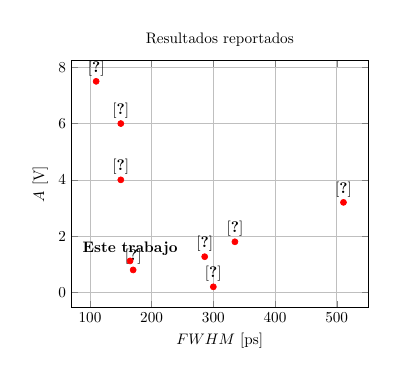
\begin{tikzpicture}[scale=0.55]
  \begin{axis}[
    xlabel={$FWHM$ [\unit{\pico\second}]},
    ylabel={$A$ [\unit{\volt}]},
    title=Resultados reportados,
    grid=both
    ]
    \addplot[
        scatter/classes={a={blue}, b={red}},
        scatter, mark=*, only marks, 
        scatter src=explicit symbolic,
        nodes near coords*={\Label},
        visualization depends on={value \thisrow{label} \as \Label} %<- added value
    ]
      table [meta=class, row sep=crcr] {
        x   y       class   label \\
        511 3.2     b       {\cite{rulikowski2004}} \\
        335 1.8     b       {\cite{rulikowski2004}} \\
        110 7.5     b       {\cite{protiva2009}} \\
        170 0.8     b       {\cite{kamal2014}} \\
        300 0.2     b       {\cite{han2002}} \\
        150 6       b       {\cite{han2005}} \\
        150 4       b       {\cite{han2005}} \\
        286 1.27    b       {\cite{oloumi2018}} \\
        165 1.12    b       {\textbf{Este trabajo}} \\
    };

  \end{axis}
\end{tikzpicture}
\end{figure}

\end{frame}

\subsection{Aplicaciones}

\begin{frame}{Aplicaciones en transmisión I}

    \begin{columns}[T]
        \begin{column}{0.5\textwidth}
            \begin{figure}[b]
                \centering
                \includegraphics[width=\textwidth]{images/passband_pulser_sim_no_amp_results.png}
                \caption{Simulación con pulso ideal y pulser sin buffer.}
            \end{figure}
            \end{column}
        \begin{column}{0.5\textwidth}
            \begin{figure}[b]
                \centering
                \includegraphics[width=\linewidth]{images/passband_pulser_sim_with_amp_result.png}
            \end{figure}
            \vspace{-0.5cm}
            \begin{figure}[b]
                \centering
                \includegraphics[width=\linewidth]{images/passband_with_measurement_result.png}
                \caption{Simulación con buffer y con pulso medido.}
            \end{figure}
        \end{column}
    \end{columns}

\end{frame}

\begin{frame}{Aplicaciones en transmisión II}

    \begin{columns}[T]
        \begin{column}{0.5\textwidth}
            \begin{figure}[b]
                \centering
                \includegraphics[width=\linewidth]{images/passband_pulses_simulations_spectrums.png}
                \label{fig:passband_spectrums_simulation}
                \caption{PSDs de pulsos simulados.}
            \end{figure}
        \end{column}
        \begin{column}{0.5\textwidth}
            \begin{figure}[b]
                \centering
                \includegraphics[width=\linewidth]{images/passband_pulses_measurement_spectrums.png}
                \label{fig:passband_spectrums_measurement}
                \caption{PSDs de simulación utilizando pulso medido.}
            \end{figure}
        \end{column}
    \end{columns}

\end{frame}

\section{Conclusiones}

\subsection{Conclusiones}

\begin{frame}{Conclusiones}
    \begin{itemize}
        \item Se logró implementar un generador de pulsos con los requisitos
            establecidos.
        \item El circuito resultante es de muy bajo costo y fácil integración en
            sistemas UWB.
        \item Se comprobó exitosamente la aplicación del generador desarrollado
            en caminos de transmisión UWB.
        \item Los resultados obtenidos son comparables o superiores con los del
            estado del arte.
    \end{itemize}
\end{frame}

\subsection{Trabajos a futuro}

\begin{frame}{Trabajos a futuro}
    \begin{itemize}
        \item Explorar mejoras al modelo del SRD o de los componentes parásitos
            para replicar los efectos observados en medición.
        \item Implementar el circuito de transmisión UWB propuesto.
        \item Simular e implementar el circuito de recepción UWB propuesto.
    \end{itemize}
\end{frame}

\begin{frame}[allowframebreaks]{Referencias}
    \bibliographystyle{ieeetr}
    \bibliography{src/mybib}
\end{frame}

\begin{frame}{}
  \centering \Huge
  \emph{Gracias por su atención.}
  \emph{¿Preguntas?}
\end{frame}

\end{document}
